\chapter{软件设计实现}\label{chap:software}

\section{NVDLA 软件工具链概述}

在前面的章节,我们略微提到过 NVDLA 的软件栈。但是在这一小节,我们将详细的介绍 NVDLA 的软件工具链。如图~\ref{fig:NVDLA Software},英伟达官方提供了完整的软件生态。

\begin{figure}[!htbp]
    \centering
    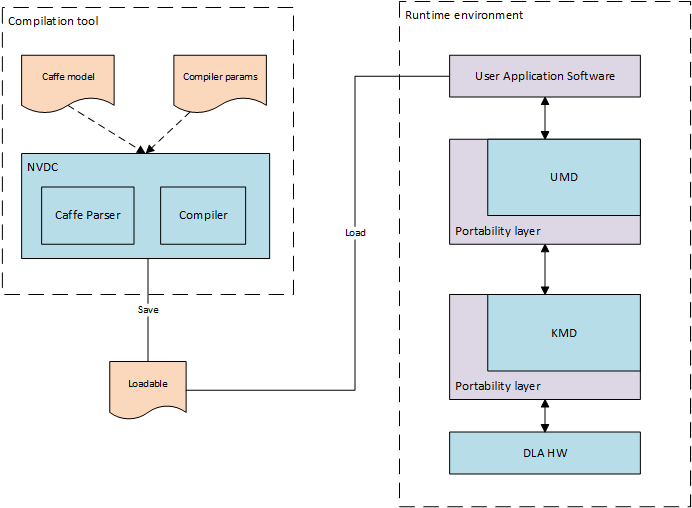
\includegraphics[width=0.7\textwidth]{software_package.png}
    \caption{NVDLA Software}
    \label{fig:NVDLA Software}
\end{figure}

Compiler 是软件工具链的前端,与硬件无关,Compiler 能够接受的参数如下:

\begin{lstlisting}
./nvdla_compiler -h
Usage: ./nvdla_compiler [-options] --prototxt <prototxt_file> --caffemodel <caffemodel_file>
where options include:
    -h                                                 print this help message
    -o <outputpath>                                    
    --profile <basic|default|performance|fast-math>    computation profile
    --cprecision <fp16|int8>                           compute precision
    --configtarget <nv_full|nv_large|nv_small>         target platform
    --calibtable <int8 calib file>                     
    --quantizationMode <per-kernel|per-filter>         
\end{lstlisting}

\begin{itemize}
    \item profile 指定了优化方案,在 Compiler 内部提供了四种优化方案,能够支持一些硬件无关的网络优化,例如算子融合、内存重用等,本设计使用默认的 fast-math,启用全部的优化选项。
    \item cprecision 指定了精度,在这里我们需要选择 int8,并且可以结合 TensorRT 生成 calibtabel 文件,如果不给出 calibtabel 参数,Compiler 内部会使用简单的量化方案,实测效果很差。
    \item configtarget 本设计选择 nv\_small,匹配本设计的 small 配置。
    \item calibtabel 需由 TensorRT 生成,将在下一小节详细介绍。
    \item quantizationMode 有两个选项,per-kernel 选项是对每一层卷积使用相同的量化参数,per-filter 则是对每一层卷积使用不同的量化参数,这需要结合 calibtabel 文件选择,在本设计中使用 per-kernel。
\end{itemize}

最终,Compiler 生成 Loadable 文件,交给 Runtime 进行加速器的调度。

Loadable 文件是 Compiler 与 Runtime 之间通信的媒介,其由 Google 开源的 FlatBuffers 序列化协议所组织,能够将对象与数据进行压缩,以便在网络中进行传输。简单来讲,我们需要在流中传输一个对象,比如网络流。一般我们需要把这个对象序列化之后才能在流中传输(例如,可以把对象直接转化为字符串),然后在接收端进行反序列化(例如把字符串解析成对象)。但是显然把对象转成字符串传输的方法效率十分低下,于是有了各种流的转换协议,FlatBuffers也是其中一种。

Runtime 与硬件紧密贴合,其又分为 UMD 和 KMD 两个部分:UMD 是用户应用,需要我们在 Linux 上编译运行,其接受 Loadable 文件并解析,最后递交一个推理任务到 KMD;KMD 是内核驱动,需要我们在构建 Linux 的时候编译,运行 Linux 的时候挂载,接受推理任务之后负责调度网络,配置寄存器,处理中断等任务。Runtime 能够接受的参数如下:

\begin{lstlisting}
./nvdla_runtime -h
Usage: ./nvdla_runtime [-options] --loadable <loadable_file>
where options include:
    -h                    print this help message
    -s                    launch test in server mode
    --image <file>        input jpg/pgm file
    --normalize <value>   normalize value for input image
    --mean <value>        comma separated mean value for input image
    --rawdump             dump raw dimg data
\end{lstlisting}

Compiler 的编译过程较简单,本设计不多介绍,Runtime 的构建过程非常复杂,将在后面的章节详细介绍。

\section{TensorRT 与模型量化}

本设计使用的 small 配置,仅支持 INT8 的推理,而 Caffe 框架仅支持 Float32 类型的训练,所以我们必须进行模型的量化。前文提到,在 Compiler 中量化需要结合英伟达公司的 TensorRT 框架。

\subsection{TensorRT 量化原理}

将高精度的浮点型转化为八比特的定点类型的量化方法,都遵循如下的公式:

$$ T_F = SF * T_I + B $$


其中$T_F$指 Float 类型的张量、$SF$指 Scale Factor、$B$指偏置 Bias,通过实验测得,Bias 去掉对精度的影响不大,最终该公式变为:

$$ T_F = SF * T_I $$

综合以上,进行神经网络的量化,本质上是求得每个参数的 Scale Factor 。最简单的量化方案是 max-max 映射:

$$ SF = \frac{|W|_{max}}{128} $$

将权重数据根据绝对值的最大值作为阈值,归一化到 -128 到 127之间,该方法针对分布均匀的权重数据是很有效果的。但是很明显,如果权重数据分布不均匀,该方法带来的精度损失很大。

TensorRT 选择的量化方法是 KL-divergence,即转化为最小化相对熵的问题。相对熵表述的就是两个分布的差异程度,在量化问题上表述的是量化前后两个分布的差异程度,而我们的问题自然而然就代表着差异最小。关于求解的算法本设计不阐述,实际上英伟达也只是公开了解决方案,但是软件算法实现并没有开源,在 TensorRT 中我们也是只能调用其封装好的链接库。

\subsection{量化步骤与精度损失}

使用 TensorRT 进行量化的宏观处理流程如下,首先准备一个校准数据集,然后对每一层进行 Float32 的推理,之后依次:

\begin{enumerate}
    \item 收集激活值的直方图;
    \item 基于不同的阀址产生不同的量化分布;
    \item 然后计算每个分布与原分布的相对熵,然后选择熵最小的一个,也就是跟原分布最像的一个;
\end{enumerate}

校准是核心部分,校准数据集可以从训练集或者验证集中采样,本设计选择从验证集中进行采样方便对比精度损失情况,关于采样多少张图片,英伟达官方建议采样 500 到 1000 张图片。

本文设计并且量化了三个网络:

\begin{enumerate}
    \item 针对 MNIST 数据集的 Lenet5
    \item 针对 CIFAR10 数据集的 Resnet18
    \item 针对 IMAGENET2012 数据集的 Resnet18
\end{enumerate}

这些网络的结构与量化样例代码详见附录,这里仅给出量化前后的精度损失情况,如表~\ref{tab:Qualifications Report}。

\begin{table}[!htbp]
    \caption{TensorRT 量化精度损失}
    \label{tab:Qualifications Report}
    \centering
    \footnotesize% fontsize
    \setlength{\tabcolsep}{4pt}% column separation
    \renewcommand{\arraystretch}{1.2}%row space 
    \begin{tabular}{lcc}
        \toprule
        \textbf{Network}      & \multicolumn{1}{l}{\textbf{Valiadation Accuracy \%}} & \multicolumn{1}{l}{\textbf{Calibration Accuracy \%}} \\
        \midrule
        Lenet5-MNIST          & 99.7                                                 & 99.5                                                 \\
        Resnet18-CIFAR10      & 90.2                                                 & 86.7                                                 \\
        Resnet18-IMAGENET2012 & 60.2                                                 & 50.5                                                 \\
        \bottomrule                   
    \end{tabular}
\end{table}

\subsection{calibtabel 生成}

使用 TensorRT 量化会生成 cache 文件,内部每一行代表每一个 layer 的 Scale Factor ,但是 NVDLA 的 Compiler 在进行量化时需要接受 Json 格式的文件,其结构如下:

\begin{lstlisting}
    {"first_conv":
        {"scale": 1.0007381439208984,
         "max": 0,
         "offset": 0,
         "min": 0
        }
    },
\end{lstlisting}

其中 first\_conv 是 Layer 的 name,遗憾的是,英伟达官方没有提供正常可用的 Cache 到 Json 转换的脚本,本设计使用 Python3 结合 PyCaffe 自行编写了 Cache 文件到 Json 文件转化的脚本,该脚本的内容详见附录。

这样,我们就可以生成针对 small 配置的 Loadable 文件,只要将 Loadable 与输入 Image 准备好,就可以使用 Runtime 自动调度加速器进行推理,接下来介绍 Runtime 的上板编译过程。

\section{Petalinux 工具介绍}

Xilinx Petalinux 是一个定制版的 Yocto 工具,包括了Linux Kernel、u-boot、device-tree、rootfs等源码、库,可以让客户很方便的生成、配置、编译及自定义。Petalinux支持Zynq UltraScale+ MPSoC、Zynq-7000全可编程SoC,以及MicroBlaze,可与Xilinx硬件设计工具Vivado协同工作,大大简化了Linux系统的开发工作。

使用PetaLinux工具,开发人员可以定制u-boot、Linux内核或Linux应用,开发者还可以通过网络或JTAG在随附的全系统仿真器 (QEMU) 或物理硬件上添加新的内核、器件驱动程序、应用和库,以及启动并测试软件协议栈,完成从系统启动到执行的所有操作。在主机端提供的PetaLinux工具包括:

\begin{itemize}
    \item 命令行界面
    \item 应用、器件驱动程序、库生成器以及开发模板
    \item 可引导的系统镜像生成器
    \item 调试代理程序
    \item GCC工具集
    \item 集成的QEMU全系统仿真器
    \item 自动化工具
    \item 支持Xilinx系统调试器
\end{itemize}

本设计将基于 Petalinux 2019.1 (Linux Kernel 版本为 4.19)完成 KMD 环境的移植与 UMD 应用的编译,由于 NVDLA 官方仓库的代码是针对 Linux Kernel 4.13 与 64位架构处理器的,其有一些函数已经在本内核函数中被废弃,还有一些操作在本设计采用的 32位 处理器上不被允许,这些问题都将在本章得到解决。

此外,Petalinux 不具备包管理工具,为了更方便开发与调试,本章将介绍 Ubuntu 16.04 的根文件系统替换方法,为板卡移植 Ubuntu 操作系统。

\section{Ubuntu 16.04 根文件系统移植}

\subsection{读取 Block Design 配置信息}

\subsection{Linux 内核裁剪}

\subsection{新增 Linux 设备树节点}

\subsection{生成 Boot 和 Image 文件}

\subsection{替换根文件系统}

\section{KMD 内核程序挂载}

\section{UMD 应用程序编译}
